\documentclass[12pt,a4paper]{article}

\usepackage{lmodern}
\usepackage[T1]{fontenc}
\usepackage[utf8]{inputenc}
\usepackage[french]{babel}

\usepackage{amsfonts}
\usepackage{amsmath}
\usepackage{amssymb}
\usepackage{amsthm}
\usepackage{array}
\usepackage{xcolor}
\usepackage{tikz}
\usepackage{pdfpages}
\usepackage{fullpage}
\usepackage{graphicx}
\usepackage{listings}
\usepackage{parskip}

\usepackage[top=2cm,bottom=2cm,left=18mm,right=18mm]{geometry}

\lstdefinestyle{darkula}{backgroundcolor=\color[HTML]{2B2B2B}, 
    basicstyle=\ttfamily\color[HTML]{A9B7C6},  
    breakatwhitespace=false,         
    breaklines=true,        
    columns=fullflexible,
    commentstyle=\color[HTML]{808080},
    frame=single, 
    framexleftmargin=6mm,  
    keepspaces=true,
	keywordstyle=\color[HTML]{CC7832},
    numbers=left,                    
    numbersep=4pt, 	
    numberstyle=\ttfamily\small\color[HTML]{6897BB},
    otherkeywords={self},
	tabsize=2,
	showspaces=false,                
    showstringspaces=false,
    showtabs=false,
    stringstyle=\color[HTML]{6A8759}
}

\lstdefinestyle{default}{basicstyle=\ttfamily,  
    commentstyle=\color[HTML]{808080},
    keywordstyle=\color[HTML]{000080},
    otherkeywords={self},
    numberstyle=\tiny\color[HTML]{6897BB},
    stringstyle=\color[HTML]{008000},
    breakatwhitespace=false,         
    breaklines=true,        
    columns=fullflexible,          
    keepspaces=true,  
    numbers=left,                    
    numbersep=5pt, 	
	tabsize=2,
	showspaces=false,                
    showstringspaces=false,
    showtabs=false
}

\lstset{
	language=Python, 
    literate={á}{{\'a}}1 {é}{{\'e}}1 {í}{{\'i}}1 {ó}{{\'o}}1 {ú}{{\'u}}1
      {Á}{{\'A}}1 {É}{{\'E}}1 {Í}{{\'I}}1 {Ó}{{\'O}}1 {Ú}{{\'U}}1
      {à}{{\`a}}1 {è}{{\`e}}1 {ì}{{\`i}}1 {ò}{{\`o}}1 {ù}{{\`u}}1
      {À}{{\`A}}1 {È}{{\'E}}1 {Ì}{{\`I}}1 {Ò}{{\`O}}1 {Ù}{{\`U}}1
      {ä}{{\"a}}1 {ë}{{\"e}}1 {ï}{{\"i}}1 {ö}{{\"o}}1 {ü}{{\"u}}1
      {Ä}{{\"A}}1 {Ë}{{\"E}}1 {Ï}{{\"I}}1 {Ö}{{\"O}}1 {Ü}{{\"U}}1
      {â}{{\^a}}1 {ê}{{\^e}}1 {î}{{\^i}}1 {ô}{{\^o}}1 {û}{{\^u}}1
      {Â}{{\^A}}1 {Ê}{{\^E}}1 {Î}{{\^I}}1 {Ô}{{\^O}}1 {Û}{{\^U}}1
      {Ã}{{\~A}}1 {ã}{{\~a}}1 {Õ}{{\~O}}1 {õ}{{\~o}}1
      {œ}{{\oe}}1 {Œ}{{\OE}}1 {æ}{{\ae}}1 {Æ}{{\AE}}1 {ß}{{\ss}}1
      {ű}{{\H{u}}}1 {Ű}{{\H{U}}}1 {ő}{{\H{o}}}1 {Ő}{{\H{O}}}1
      {ç}{{\c c}}1 {Ç}{{\c C}}1 {ø}{{\o}}1 {å}{{\r a}}1 {Å}{{\r A}}1
      {€}{{\euro}}1 {£}{{\pounds}}1 {«}{{\guillemotleft}}1
      {»}{{\guillemotright}}1 {ñ}{{\~n}}1 {Ñ}{{\~N}}1 {¿}{{?`}}1
}

\author{Lucas David \& Théo Legras}

\title{Rapport de projet de reconnaissance d'images}
\date{}

\begin{document}
\maketitle

\section{Implémentation et utilisation du classificateur à distance minimum (DMIN)}

On choisi d'implémenter ce classificateur sous forme d'une classe, ceci étant le plus courant et le plus pratique pour encapsuler les comportements et stocker les données nécessaires (extrait du fichier {\textbf{\ttfamily dmin.py}):
\begin{lstlisting}[style=darkula]
import numpy as np

class DMIN:
	def __init__(self):
		self.data = np.array([])
		self.label = np.array([])
		self.n_samples = 0

	def fit(self, data, label):
		self.data = data
		self.label = label
		self.n_samples = len(set(label))
		return self
		
	def predict(self, data):
		return [self.label[np.argmin(np.sum(np.subtract(self.data, data[iterator]) ** 2, axis=1))] for iterator in range(0, len(data))]

	def score(self, data, label):
		return np.count_nonzero(self.predict(data) == label) / len(data)
\end{lstlisting}

L'utilisation se résumera à l'instanciation de \lstinline[style=default]|DMIN| à l'appel de \lstinline[style=default]|DMIN.fit| et selon l'usage l'appel de \lstinline[style=default]|DMIN.predict| et \lstinline[style=default]|DMIN.score|.
En particulier, on peut donc déterminer le taux de réussite via la fonction membre \lstinline[style=default]|DMIN.score(<données à tester>, <labels correspondants>)|.

Dans le cas de nos données de développement, on obtient un score de 68,80\% pour une exécution de 96,45 secondes.
Il est toujours intéressant de noter que si on teste l'ensemble d'entraînement, on obtient le score parfait... On verra plus tard que ce n'est pas le cas de tous les algorithmes car cela peut être un indicateur d'\textit{overfitting} (du surapprentissage ou de la surinterprétation), c'est-à-dire correspond trop étroitement aux données.

\section{Utilisation de l'analyse en composantes principales (PCA) et application à DMIN}

L'utilisation de l'Implémentation de la PCA (\lstinline[style=default]|sklearn.decompostion.PCA|) est plutôt simple. 
On peut choisir via le paramêtre \lstinline[style=default]|n_components| le nombre de dimensions à garder, \linebreak[4] si $0 \leq$  \lstinline[style=default]|n_components| $< 1$, on indique la proportion des données à garder en variance (\%).

Nous nous choisissons de faire nos tests en modulant en variance plus qu'en nombre de dimensions car la notion de variance peut être mise en parallèle avec la perte de précision à postériori de la PCA.
De plus cela permet d'écarter les cas de réductions dans des nombres dimensions proches (e.g. passer de 760 dims. à 700 dims. ne signifie pas grand chose alors que de 100 dims. à 40 dims. à un impact visible). Effectivement, selon le modèle on n'obtiendra pas la même courbe ``Variance des données par rapport aux nombres de dimensions'' et ce n'est généralement pas linéaire.

Globalement, nous appliquons dans les grandes ligne la PCA et DMIN sur les données réduites comme suit:
\begin{lstlisting}[style=darkula]
import numpy as np
from sklearn.decompostion import PCA

X = np.load('data/trn_img.npy')
Y = np.load('data/trn_lbl.npy')
devX = np.load('data/dev_img.npy')
devY = np.load('data/dev_lbl.npy')

pca = PCA(n_components=0.5) # Ici on garde 50% de la variance des données.
reducedX = pca.fit_transform(X) # On colle au modèle et on transforme X.
print('Dimensions: {}'.format(reducedX)) # On peut afficher le nombre de dimension en valeur.
reducedDevX = pca.transform(reducedDevX) # On transforme devX.

dmin = DMIN() # On utilise DMIN.
dmin.fit(reducedX, Y)
print('Score: {}'.format(dmin.score(reducedDevX, devY)))

\end{lstlisting}

En terme de vitesse d'exécution initialiser la PCA et l'appliquer se fait en temps très raisonnable et permet de réduire drastiquement le temps d'exécution de DMIN. De plus, on remarquera que le fait d'appliquer la PCA améliore un peu le score lorsque l'on garde jusqu'à 50\% de la variance des données, on peut se douter que le fait de retirer certaine dimensions à diminuer en quelques sortes le bruit de l'image néfaste dans le cas de l'algorithme DMIN.

\begin{tabular}{m{8,5cm}m{}}
    \sffamily\small\centering
    \begin{tabular}{|c|c|c|c|c|}
        \hline
        \tiny n (\%) & \tiny n (dims) & \tiny Execution time PCA & \tiny Score DMIN & \tiny Execution time DMIN \\
        \hline
        0,05         & 1              & 0,855s                   & 22,60\%          & 0,149s     \\
        0,1          & 1              & 0,809s                   & 22,60\%          & 0,157s     \\
        0,15         & 1              & 0,776s                   & 22,60\%          & 0,149s     \\
        0,2          & 1              & 0,779s                   & 22,60\%          & 0,155s     \\
        0,25         & 1              & 0,775s                   & 22,60\%          & 0,158s     \\
        0,3          & 2              & 0,791s                   & 45,18\%          & 0,207s     \\
        0,35         & 2              & 0,806s                   & 45,18\%          & 0,212s     \\
        0,4          & 2              & 0,772s                   & 45,18\%          & 0,21s      \\
        0,45         & 2              & 0,781s                   & 45,18\%          & 0,209s     \\
        0,5          & 3              & 0,780s                   & 56,30\%          & 0,256s     \\
        0,55         & 4              & 0,800s                   & 65,44\%          & 0,314s     \\
        0,6          & 5              & 0,821s                   & 68,64\%          & 0,329s     \\
        0,65         & 6              & 0,844s                   & 71,42\%          & 0,379s     \\
        0,7          & 9              & 0,814s                   & 76,28\%          & 0,501s     \\
        0,75         & 14             & 0,790s                   & 78,12\%          & 0,687s     \\
        0,8          & 24             & 0,806s                   & 80,50\%          & 1,076s     \\
        0,85         & 42             & 0,804s                   & 81,84\%          & 1,837s     \\
        0,9          & 82             & 0,807s                   & 82,56\%          & 4,129s     \\
        0,95         & 182            & 0,821s                   & 82,36\%          & 11,542s    \\
        1            & 784            & --                       & 68,80\%          & 96,458s    \\
        \hline
    \end{tabular} & 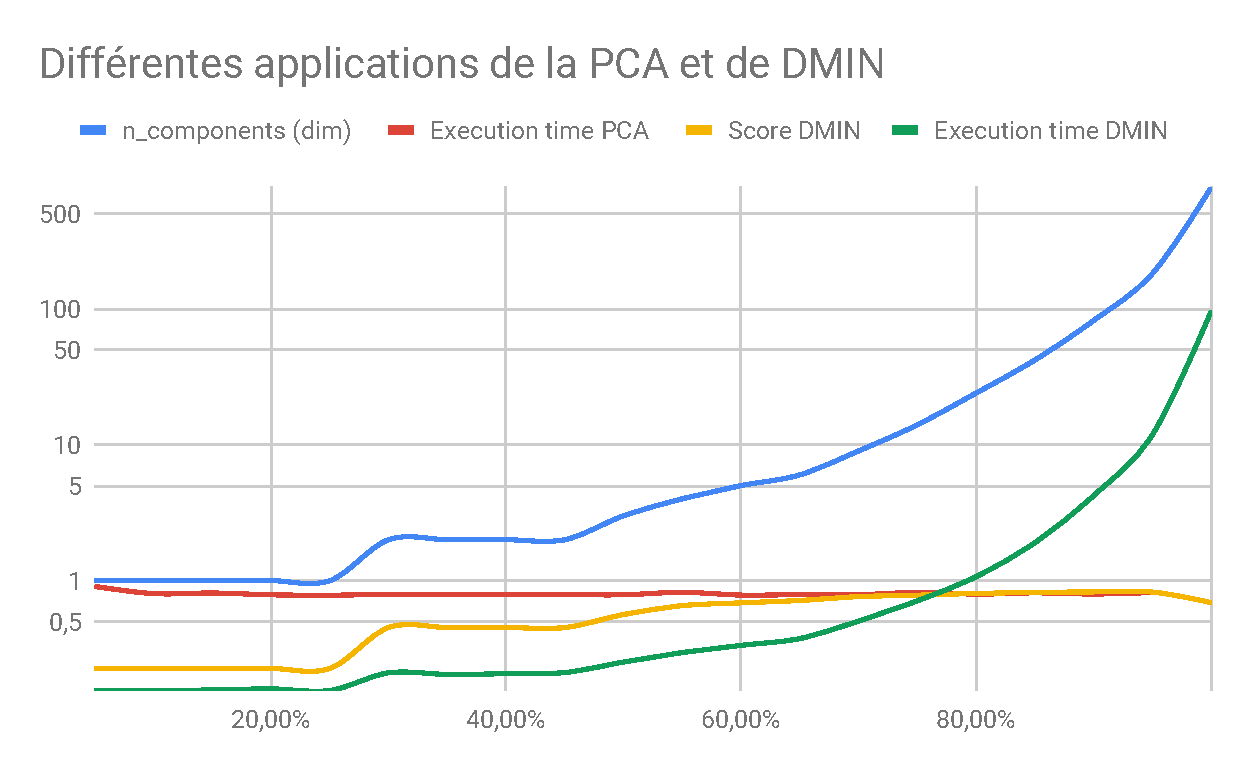
\includegraphics[scale=0.45]{PCA+DMIN.pdf} \\
\end{tabular}

\section{Choix des implémentations et utilisations des classificateurs et paramètres}



Pour commencer notre analyse nous avons choisis d'appliquer la PCA à différentes variance sur différentes méthodes proposer afin d'en analyser les résultats et de proposer un segment d'utilisation optimal de la PCA sur ce modèle. Pour ce faire, nous avons créer une fonction générique \lstinline[style=default]|BenchmarkPCA| permettant de tester les classificateurs fournies en paramètre et d'en extraire les temps d'exécutions et scores correspondants.
\begin{lstlisting}[style=darkula]
def BenchmarkPCA(csvfile, n_range, algorithms):
	csvwriter = csv.writer(csvfile, delimiter=';')
	first_row = ['n_components (%)', 'n_components (dims)', 'Execution time PCA']
	for algorithm in algorithms:
		first_row.extend(['Score {}'.format(algorithm), 'Execution time {}'.format(algorithm)])
	csvwriter.writerow(first_row)

	# On fait une PCA pour chaque valeur
	for n in n_range:
		print('PCA with n_components={}:'.format(n))
		start = time.time()
		pca = PCA(n_components=n)
		reducedX = pca.fit_transform(X)
		reducedDevX = pca.transform(devX)
		end = time.time()
		print('PCA both fit and transform (on training and dev data) processed in {} sec...'.format(end - start))
		print('\tn_components={} reduce 784 dimensions to {} dimensions.\n'.format(n, np.shape(reducedX)[1]))
		csvrow = [n, np.shape(reducedX)[1], end - start]
		
		# On test chaque algorithm de la liste
		for algorithm in algorithms:
			print('Testing {} algorithm:'.format(algorithm))
			start = time.time()
			if algorithm == SVC:
				# Le mode par défaut dans la prochaine version est avec gamma='scale' et on voit la différence.
				algorithm_instance = algorithm(gamma='scale')
			else:
				algorithm_instance = algorithm()
			algorithm_instance.fit(reducedX, Y)
			algorithm_score = algorithm_instance.score(reducedDevX, devY)
			end = time.time()
			print('Score: {}'.format(algorithm_score))
			print('Execution time: {}\n'.format(end - start))
			csvrow.extend([algorithm_score, end - start])
		csvwriter.writerow(csvrow)
\end{lstlisting}

{\sffamily\scriptsize\centering
\begin{tabular}{|*{13}{c|}}
    \hline
    \tiny n (\%) & \tiny $\frac{\text{Score}^{2}}{\text{Exec. time DMIN}}$ & \tiny Score SVC & \tiny Exec. time SVC & \tiny $\frac{\text{Score}^{2}}{\text{Exec. time SVC}}$ & \tiny Score neighbors & \tiny Exec. time neighbors & \tiny $\frac{\text{Score}^{2}}{\text{Execution time neighbors}}$ & \tiny Avg $\frac{\text{Score}^{2}}{\text{Execution time}}$ \\
    \hline
    5,00\%  & 0,33 & 31,94\% & 3,440s  & 0,01 & 25,18\% & 0,082s  & 0,77 & 0,37 \\
    10,00\% & 0,33 & 31,94\% & 3,421s  & 0,01 & 25,18\% & 0,082s  & 0,77 & 0,37 \\
    15,00\% & 0,33 & 31,94\% & 3,467s  & 0,01 & 25,18\% & 0,087s  & 0,73 & 0,35 \\
    20,00\% & 0,32 & 31,94\% & 3,432s  & 0,01 & 25,18\% & 0,084s  & 0,75 & 0,36 \\
    25,00\% & 0,33 & 31,94\% & 3,439s  & 0,01 & 25,18\% & 0,083s  & 0,77 & 0,37 \\
    30,00\% & 0,97 & 54,58\% & 1,886s  & 0,09 & 51,38\% & 0,084s  & 3,13 & 1,40 \\
    35,00\% & 1,00 & 54,58\% & 1,896s  & 0,09 & 51,38\% & 0,085s  & 3,11 & 1,40 \\
    40,00\% & 0,99 & 54,58\% & 1,891s  & 0,09 & 51,38\% & 0,084s  & 3,14 & 1,40 \\
    45,00\% & 0,97 & 54,58\% & 1,909s  & 0,09 & 51,38\% & 0,084s  & 3,13 & 1,40 \\
    50,00\% & 1,26 & 63,52\% & 1,637s  & 0,16 & 61,58\% & 0,089s  & 4,27 & 1,90 \\
    55,00\% & 1,45 & 70,22\% & 1,476s  & 0,23 & 68,96\% & 0,095s  & 5,00 & 2,23 \\
    60,00\% & 1,41 & 73,18\% & 1,430s  & 0,27 & 72,18\% & 0,106s  & 4,92 & 2,20 \\
    65,00\% & 1,36 & 75,06\% & 1,400s  & 0,30 & 74,72\% & 0,114s  & 4,91 & 2,19 \\
    70,00\% & 1,15 & 80,20\% & 1,446s  & 0,36 & 79,06\% & 0,142s  & 4,41 & 1,97 \\
    75,00\% & 0,86 & 82,44\% & 1,627s  & 0,34 & 81,28\% & 0,203s  & 3,25 & 1,48 \\
    80,00\% & 0,61 & 84,34\% & 1,965s  & 0,31 & 82,32\% & 0,316s  & 2,14 & 1,02 \\
    85,00\% & 0,35 & 85,38\% & 2,725s  & 0,23 & 83,64\% & 0,557s  & 1,26 & 0,61 \\
    90,00\% & 0,16 & 86,18\% & 4,532s  & 0,14 & 83,70\% & 1,322s  & 0,53 & 0,28 \\
    95,00\% & 0,06 & 86,28\% & 9,333s  & 0,07 & 83,36\% & 3,800s  & 0,18 & 0,10 \\
    100\%   & 0,00 & 86,10\% & 39,329s & 0,02 & 82,98\% & 51,104s & 0,01 & 0,01 \\
    \hline
\end{tabular}}

\end{document}